\section{A curious example}

We have seen the power of the method of least squares: for systems without direct solutions we can always find least squares solutions. The embodiment of this capability is the pseudoinverse which orthogonally projects the data vector down onto the range thereby finding the solution in the range closest to the data. Here we present a curious example as a probe of the pseudoinverse in the method of least squares which synthesizes several important concepts.

Consider the linear system given by this:
\begin{equation*}
  \ls
\end{equation*}
If the matrix $\A{}$ describes two intersecting lines, the system has a classic inverse and the least squares solution represents the intersection point. If the system does not have classic inverse, it has a pseudoinverse and a least squares solution. If the matrix $\A{}$ describes two parallel lines what does this solution represent?

We are begging the question: where do two parallel lines meet in the plane $\real{2}$?

Three cases follow:
\begin{enumerate}
\item Two lines with different slopes: one intersection. The linear system $ls$ has a direct solution. The least squares solution is the direct solution. The least squares solution is the point where the lines intersect.
\item Three lines each with different slopes: three distinct intersection. The linear system has no direct solution. The least squares solution is ``in the triangle.'' 
\item Two lines with the same slope: there is no intersection. What does the least squares solution mean?
\end{enumerate}

%%
\subsection{Unique intersection}

%%
\subsection{Distinct intersections}

%%
\subsection{No intersection}
Consider two functions
\begin{equation}3
\begin{split}
  f_{1}(x) &= x,\\
  f_{2}(x) &= x + 1,
  \label{eq:curious:no:system}
\end{split}
\end{equation}
which define two parallel lines with unit offset. We know the lines do not cross, yet we also know the method of least squares will create a solution point. Where is this solution point?

%%
\subsection{The problem}
The linear system is given by this
\begin{equation}
  \begin{split}
    \lsa\\
    \mat{cc}{1&1\\1&1}\mat{c}{x\\y} &= \mat{c}{0\\1}.
  \end{split}
\end{equation}There is one independent row vector $r_{1}$:
\begin{equation}
  \mat{cc}{1&1\\\hline1&1} = \mat{c}{r_{1}^{\mathrm{T}}\\\hline r_{1}^{\mathrm{T}}}, \qquad r_{1}=\mat{c}{1\\1}.
\end{equation}
The orthogonal complement vectors are given by this
\begin{equation}
  r_{1}^{\perp} = \alpha\mat{r}{-1\\1}, \quad \alpha \in \cmplx{}.
\end{equation}
Without any loss of generality, set
\begin{equation}
  \alpha = 1.
\end{equation}
The candidate domain matrix then
\begin{equation}
  \X{} = 
\stwo
\left[
\begin{array}{r >{\columncolor{ltgray}}r}
  1 & -1 \\
  1 &  1
\end{array}
\right]
.
\end{equation}

In a similar fashion there is one independent column vector $c_{1}$:
\begin{equation}
  \mat{c|c}{1&1\\1&1} = \mat{c|c}{c_{1}&c_{1}}, \qquad c_{1}=\mat{c}{1\\1}.
\end{equation}
While this has the same value as the vector $r_{1}$, remember that the row vector $r_{1}$ is in the domain (solution space) and the column vector is in the codomain $c_{1}$ (measurement space).

Location aside, the same image vector allows us to use the same perpendicular complement. The result is the codomain matrix
\begin{equation}
  \Y{} = 
\stwo
\left[
\begin{array}{r >{\columncolor{ltgray}}r}
  1 & -1 \\
  1 &  1
\end{array}
\right]
.
\end{equation}

The lone eigenvalue comes from this relationship:
\begin{equation}
  \begin{split}
    \A{} \X{}_{*,1} &= \sigma_{1} \Y{}_{*,1},\\
    \frac{2}{\sqrt{2}}
    \mat{c}{1\\1} &= \frac{\sigma_{1}}{\sqrt{2}}
    \mat{c}{1\\1}.
  \end{split}
\end{equation}

Therefore $\sigma_{1} = 2$ and we can write the SVD for the target matrix:
\begin{equation}
  \begin{split}
     \svda{T}\\
     \mat{cc}{1&1\\1&1} &= 
     \stwo
\left[
\begin{array}{r >{\columncolor{ltgray}}r}
  1 & -1 \\
  1 &  1
\end{array}
\right]
     \mat{c|c}{2&0\\\hline 0&0}
     \stwo \mat{rr}{1&1\\\rowcolor{ltgray}-1&1}.
  \end{split}
\end{equation}

The point of the decomposition was to assemble the pseudoinverse:
\begin{equation}
  \begin{split}
     \mpgia{T}\\
      \rtwo \mat{cc}{1&1\\1&1} &= 
\stwo
\left[
\begin{array}{r >{\columncolor{ltgray}}r}
  1 & -1 \\
  1 &  1
\end{array}
\right]
     \mat{c|c}{\frac{1}{2}&0\\[3pt]\hline 0&0}
     \stwo \mat{rr}{1&1\\\rowcolor{ltgray}-1&1}.
  \end{split}
\end{equation}

The general solution to the least squares problem is written as the following:
\begin{equation}
\boxed{
  \begin{array}{rccccc}
    x_{gen} &=& x_{p} &\oplus& x_{h},\\[7pt]
      &=& \A{+}b &\oplus& \alpha \X{}_{*,2}, & \alpha\in\cmplx{}\\[7pt]
      &=& \frac{1}{4}\mat{r}{1\\1} &\oplus& \alpha \mat{r}{-1\\1}\\[17pt]
      &=& \textit{point} &\oplus& \textit{line}
  \end{array}
}
\label{eq:simple:fullsoln}
\end{equation}

\begin{figure}[htbp] %  figure placement: here, top, bottom, or page
   \centering
   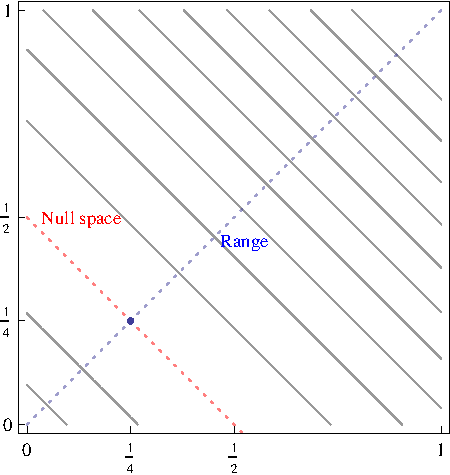
\includegraphics[ ]{pdf/lsq/curiousspaces} 
   \caption[The domain holds the contours of equal error norm]{The domain holds the contours of equal error norm. The particular solution $x_{p}=\Ap b$ will always be on the range $\rng{\A{}}$, here a dotted blue line through the origin. The null space is orthogonal to the range. The red dotted line through the solution point shows projections into the null space.}
   \label{fig:curious:no:contour}
\end{figure}

Consider an arbitrary data point
\begin{equation}
  b = \mat{c}{\alpha \\ \beta}
  \label{eq:curious:no:data}
\end{equation}
and consider the form of the solution vector $x$. Since we have the pseudoinverse we can pose the arbitrary solution immediately:
\begin{equation}
  \xtwo = \Ap b = \rfour \mat{cc}{1&1\\1&1}\mat{c}{\alpha \\ \beta} = \rfour\mat{cc}{\alpha+\beta\\\alpha+\beta}.
\end{equation}

\begin{figure}[htbp] %  figure placement: here, top, bottom, or page
   \centering
   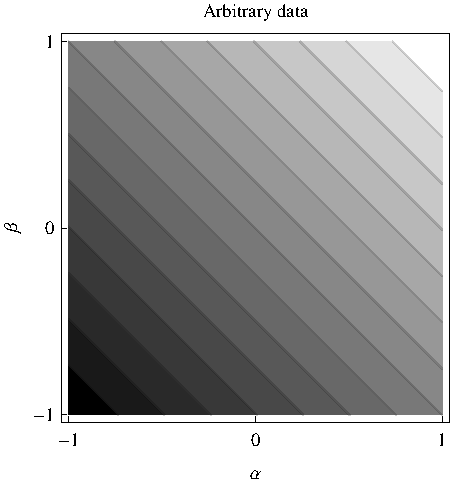
\includegraphics[ ]{pdf/lsq/curiousxy} 
   \caption[The $2-$norm of the error]{The $2-$norm of the error for the linear system in equation \eqref{eq:curious:no:system} with the arbitrary data equation \eqref{eq:curious:no:data}. Each contour - here a straight line - represents a locus of points of equal error norm. They also represent the null space. Therefore the line through the origin which is perpendicular to the null space is the range. We cannot ascertain where the solution point is from looking at this graph.}
   \label{fig:curious:no:arbitrary}
\end{figure}
\clearpage
\begin{table}[htdp]
\begin{center}
\begin{tabular}{ccc}
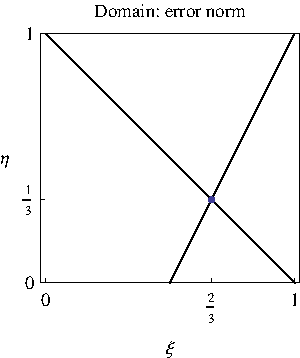
\includegraphics[ width = 1.5in ]{pdf/lsq/direct_fcns} &
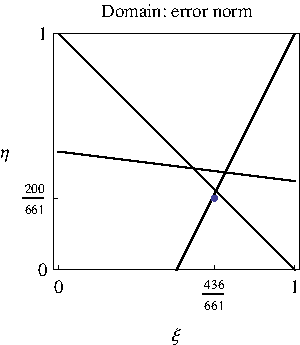
\includegraphics[ width = 1.5in ]{pdf/lsq/three_fcns}  &
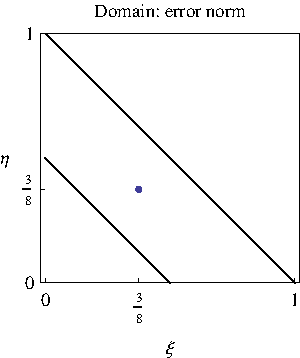
\includegraphics[ width = 1.5in ]{pdf/lsq/parallel_fcns}\\
$y_{1}(x) = -x+1$ & $y_{1}(x) = -x+1$ & $y_{1}(x) = -x+1$\\
$y_{2}(x) = 2x-1$ & $y_{2}(x) = 2x-1$ & $y_{4}(x) = -x+\frac{1}{2}$\\
 & $y_{3}(x) = -\frac{1}{8}x+\frac{3}{2}$ \\
\textellipsis & \textellipsis & \textellipsis \\
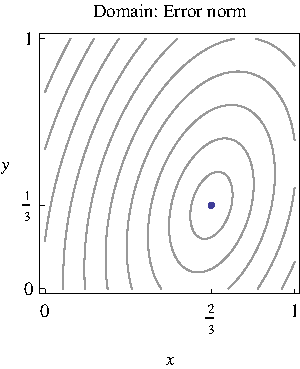
\includegraphics[ width = 1.5in ]{pdf/lsq/direct_error} &
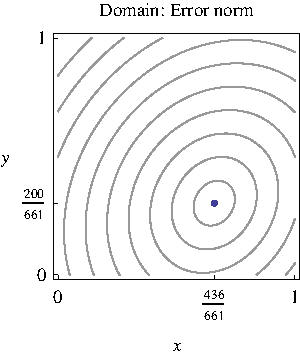
\includegraphics[ width = 1.5in ]{pdf/lsq/three_error}  &
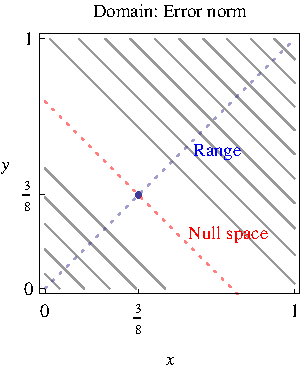
\includegraphics[ width = 1.5in ]{pdf/lsq/parallel_error}\\
\textellipsis & \textellipsis & \textellipsis \\
$\A{} = \mat{rr}{1&1\\-2&1}$ &
$\A{} = \mat{rr}{1&1\\-2&1\\1/8&3/8}$ &
$\A{} = \mat{cc}{1&1\\1&1}$ \\
\textellipsis & \textellipsis & \textellipsis \\
$\Ap = \AinvB = $ &
$\Ap = \AinvL = $ &
$\Ap = $ \\
$\rthree\mat{rr}{2&-1\\1&1}$ &
$\frac{1}{1322}\mat{rrr}{324&-492&122\\373&217&498}$ &
$\frac{1}{4}\mat{cc}{1&1\\1&1}$ \\
\textellipsis & \textellipsis & \textellipsis \\
\textellipsis & \textellipsis & \textellipsis \\
\end{tabular}
\end{center}
\caption{default}
\label{tab:curious:all}
\end{table}%

%%
\subsection{Interpretation}


\endinput